\begin{table*}[t]
\centering
\caption{\textbf{Ablation studies on the components of CCS.} The best and second-best performances are shown in bold and underline, respectively.}
\resizebox{\textwidth}{!}{
\begin{tabular}{lcccccccc}
\toprule
\multirow{2}{*}{\textbf{Methods}} & \multicolumn{3}{c}{\textbf{General QA}} & \multicolumn{4}{c}{\textbf{Multi-Hop QA}} & \multirow{2}{*}{\textbf{Avg.}} \\
\cmidrule(lr){2-4} \cmidrule(lr){5-8}
 & \textbf{NQ}$^\dagger$ & \textbf{TriviaQA}$^*$ & \textbf{PopQA}$^*$ & \textbf{HotpotQA}$^\dagger$ & \textbf{2wiki}$^*$ & \textbf{Musique}$^*$ & \textbf{Bamboogle}$^*$ & \\
\midrule
Actions + Observations + Final Response & \underline{0.700} & 0.852 & \underline{0.618} & 0.543 & 0.476 & 0.202 & \underline{0.536} & 0.561 \\
Actions + Observations  & 0.679 & 0.852 & 0.598 & 0.526 & 0.474 & 0.201 & 0.488 & 0.545 \\
Observations & 0.691 & \underline{0.866} & 0.610 & \underline{0.589} & \textbf{0.588} & \underline{0.225} & 0.520 & \underline{0.584} \\
Masked Actions + Observations  & \textbf{0.712} & \textbf{0.880} & \textbf{0.639} & \textbf{0.598} & \underline{0.567} & \textbf{0.239} & \textbf{0.608} & \textbf{0.606} \\
\bottomrule
\end{tabular}
}
\label{tbl:ablation}
\end{table*}
\begin{figure*}[!t]
    \centering
    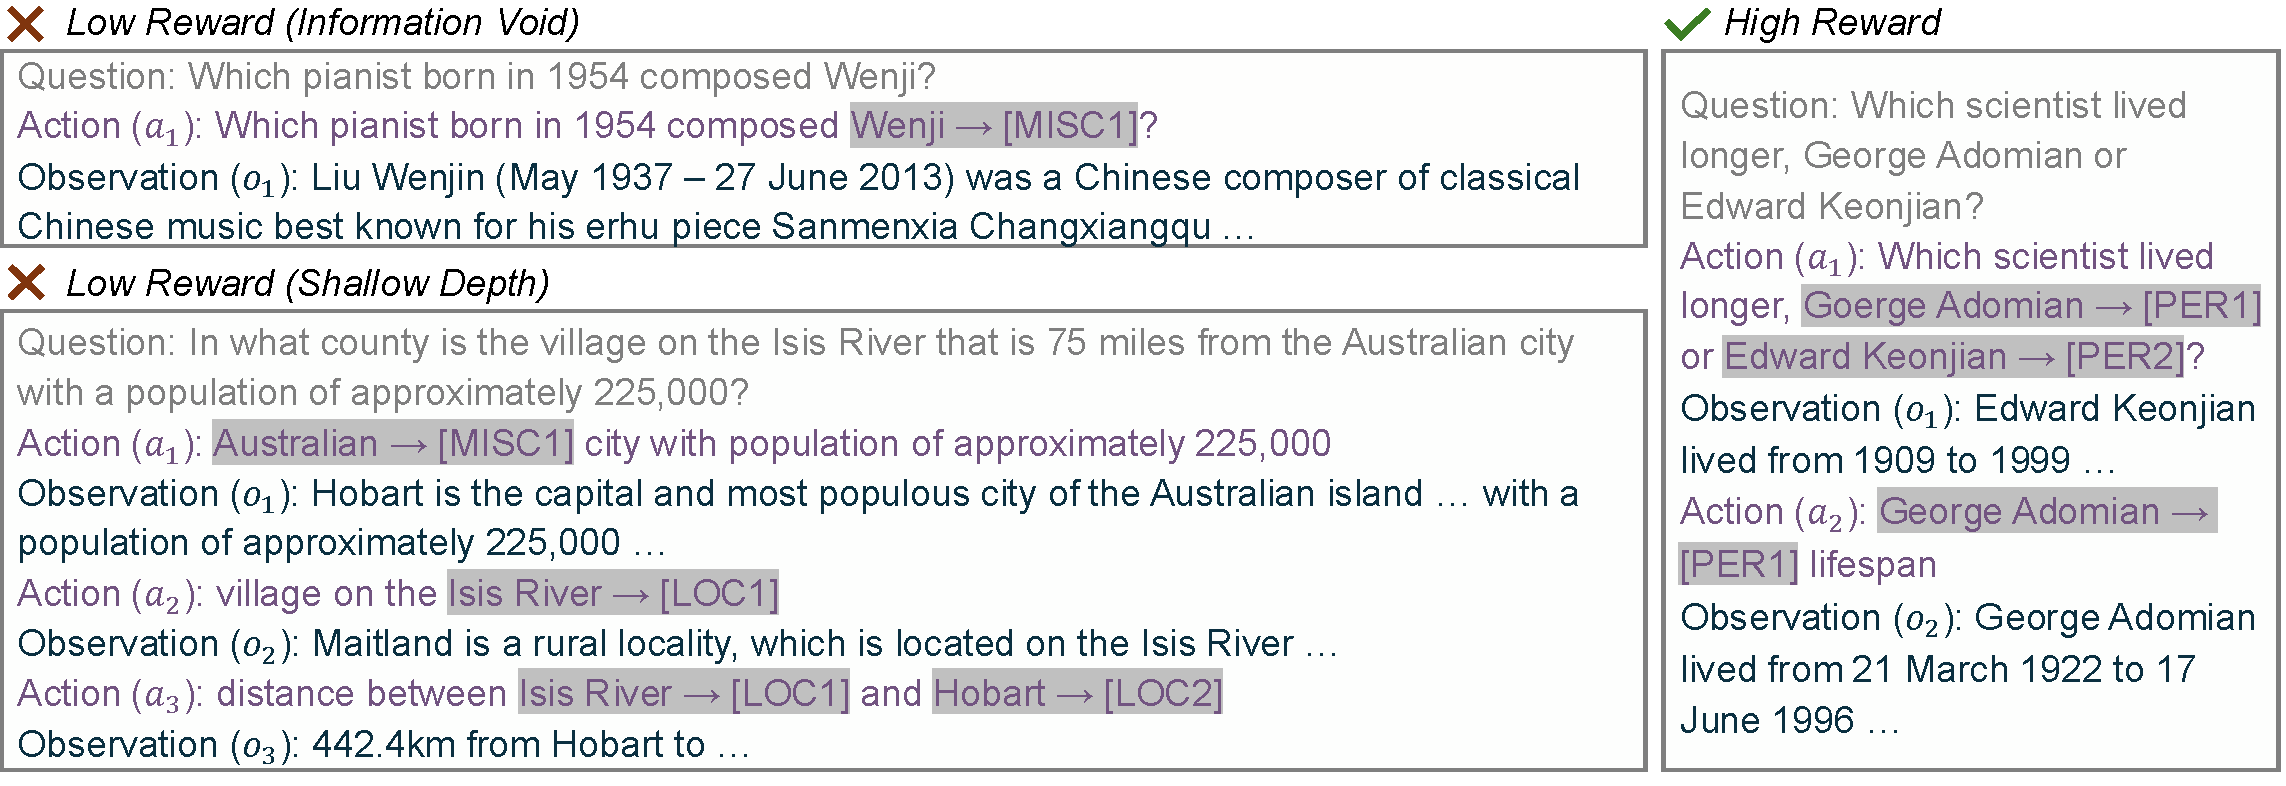
\includegraphics[width=1\linewidth]{img/ccs_qualitative_analysis.pdf}
    \caption{\textbf{Qualitative analysis of search trajectories.} CCS assigns low rewards to trajectories exhibiting (a) Information Void, where the retrieved observations fail to satisfy key entity constraints, and (b) Shallow Depth, where the agent fails to complete the full multi-hop search scaffold. By contrast, high rewards are assigned only to trajectories that preserve both the search structure and the supporting observations needed to faithfully reconstruct the original question. Masked spans are highlighted in gray.}
    \label{fig:qualitative_analysis}
\end{figure*}

% \vspace{-0.1in}
\section{Analysis}

% \vspace{-0.1in}
\subsection{Ablation Study}
% \vspace{-0.1in}
We conduct an ablation study to evaluate the role of the proposed information bottlenecks. As shown in \Cref{tbl:ablation}, variants that expose the reconstructor to unfiltered lexical cues---either by including the final response or by using unmasked actions---perform worse than the CCS bottleneck design (Masked Actions + Observations), with average scores of 0.561 and 0.545, respectively. This suggests that both the final response and raw search queries introduce shortcut signals that weaken the intended training objective.
Using observations alone yields an average score of 0.584, which remains below the 0.606 achieved by the CCS bottleneck design. This performance gap indicates that masked actions contribute more than simply removing lexical leakage: they preserve useful structural intent that helps the reconstructor interpret the observations within a specific investigative context. Overall, these results show that the proposed bottlenecks are effective not only because they suppress surface-level shortcuts, but also because they retain the structural signals needed for faithful reconstruction.

% \vspace{-0.1in}
\subsection{Qualitative Investigation}
% \vspace{-0.1in}
Qualitative analysis in \Cref{fig:qualitative_analysis} further illustrates how CCS assigns rewards based on the quality of the search trajectory. In the \emph{Information Void} case, the agent retrieves observations that are lexically related to the question (``Liu \texttt{Wenjin}'') but fail to match its key entity constraints (``composed \texttt{Wenji}''). As a result, the trajectory does not preserve the information needed to recover the original question, leading to low reconstruction fidelity and thus a low reward.
In the \emph{Shallow Depth} case, the agent follows an incomplete search scaffold and fails to complete the full multi-hop chain required by the question. Although it identifies an intermediate entity (e.g., ``Hobart''), the trajectory does not gather the additional results needed to resolve the remaining constraints (e.g., the ``county'' in question). Consequently, the reconstructor cannot recover the full relational structure of the original question, and the trajectory receives a low reward. Together, these examples show that CCS rewards trajectories only when they preserve both the search structure and the supporting observations needed for faithful reconstruction.


\begin{figure*}[!t]
    \centering
    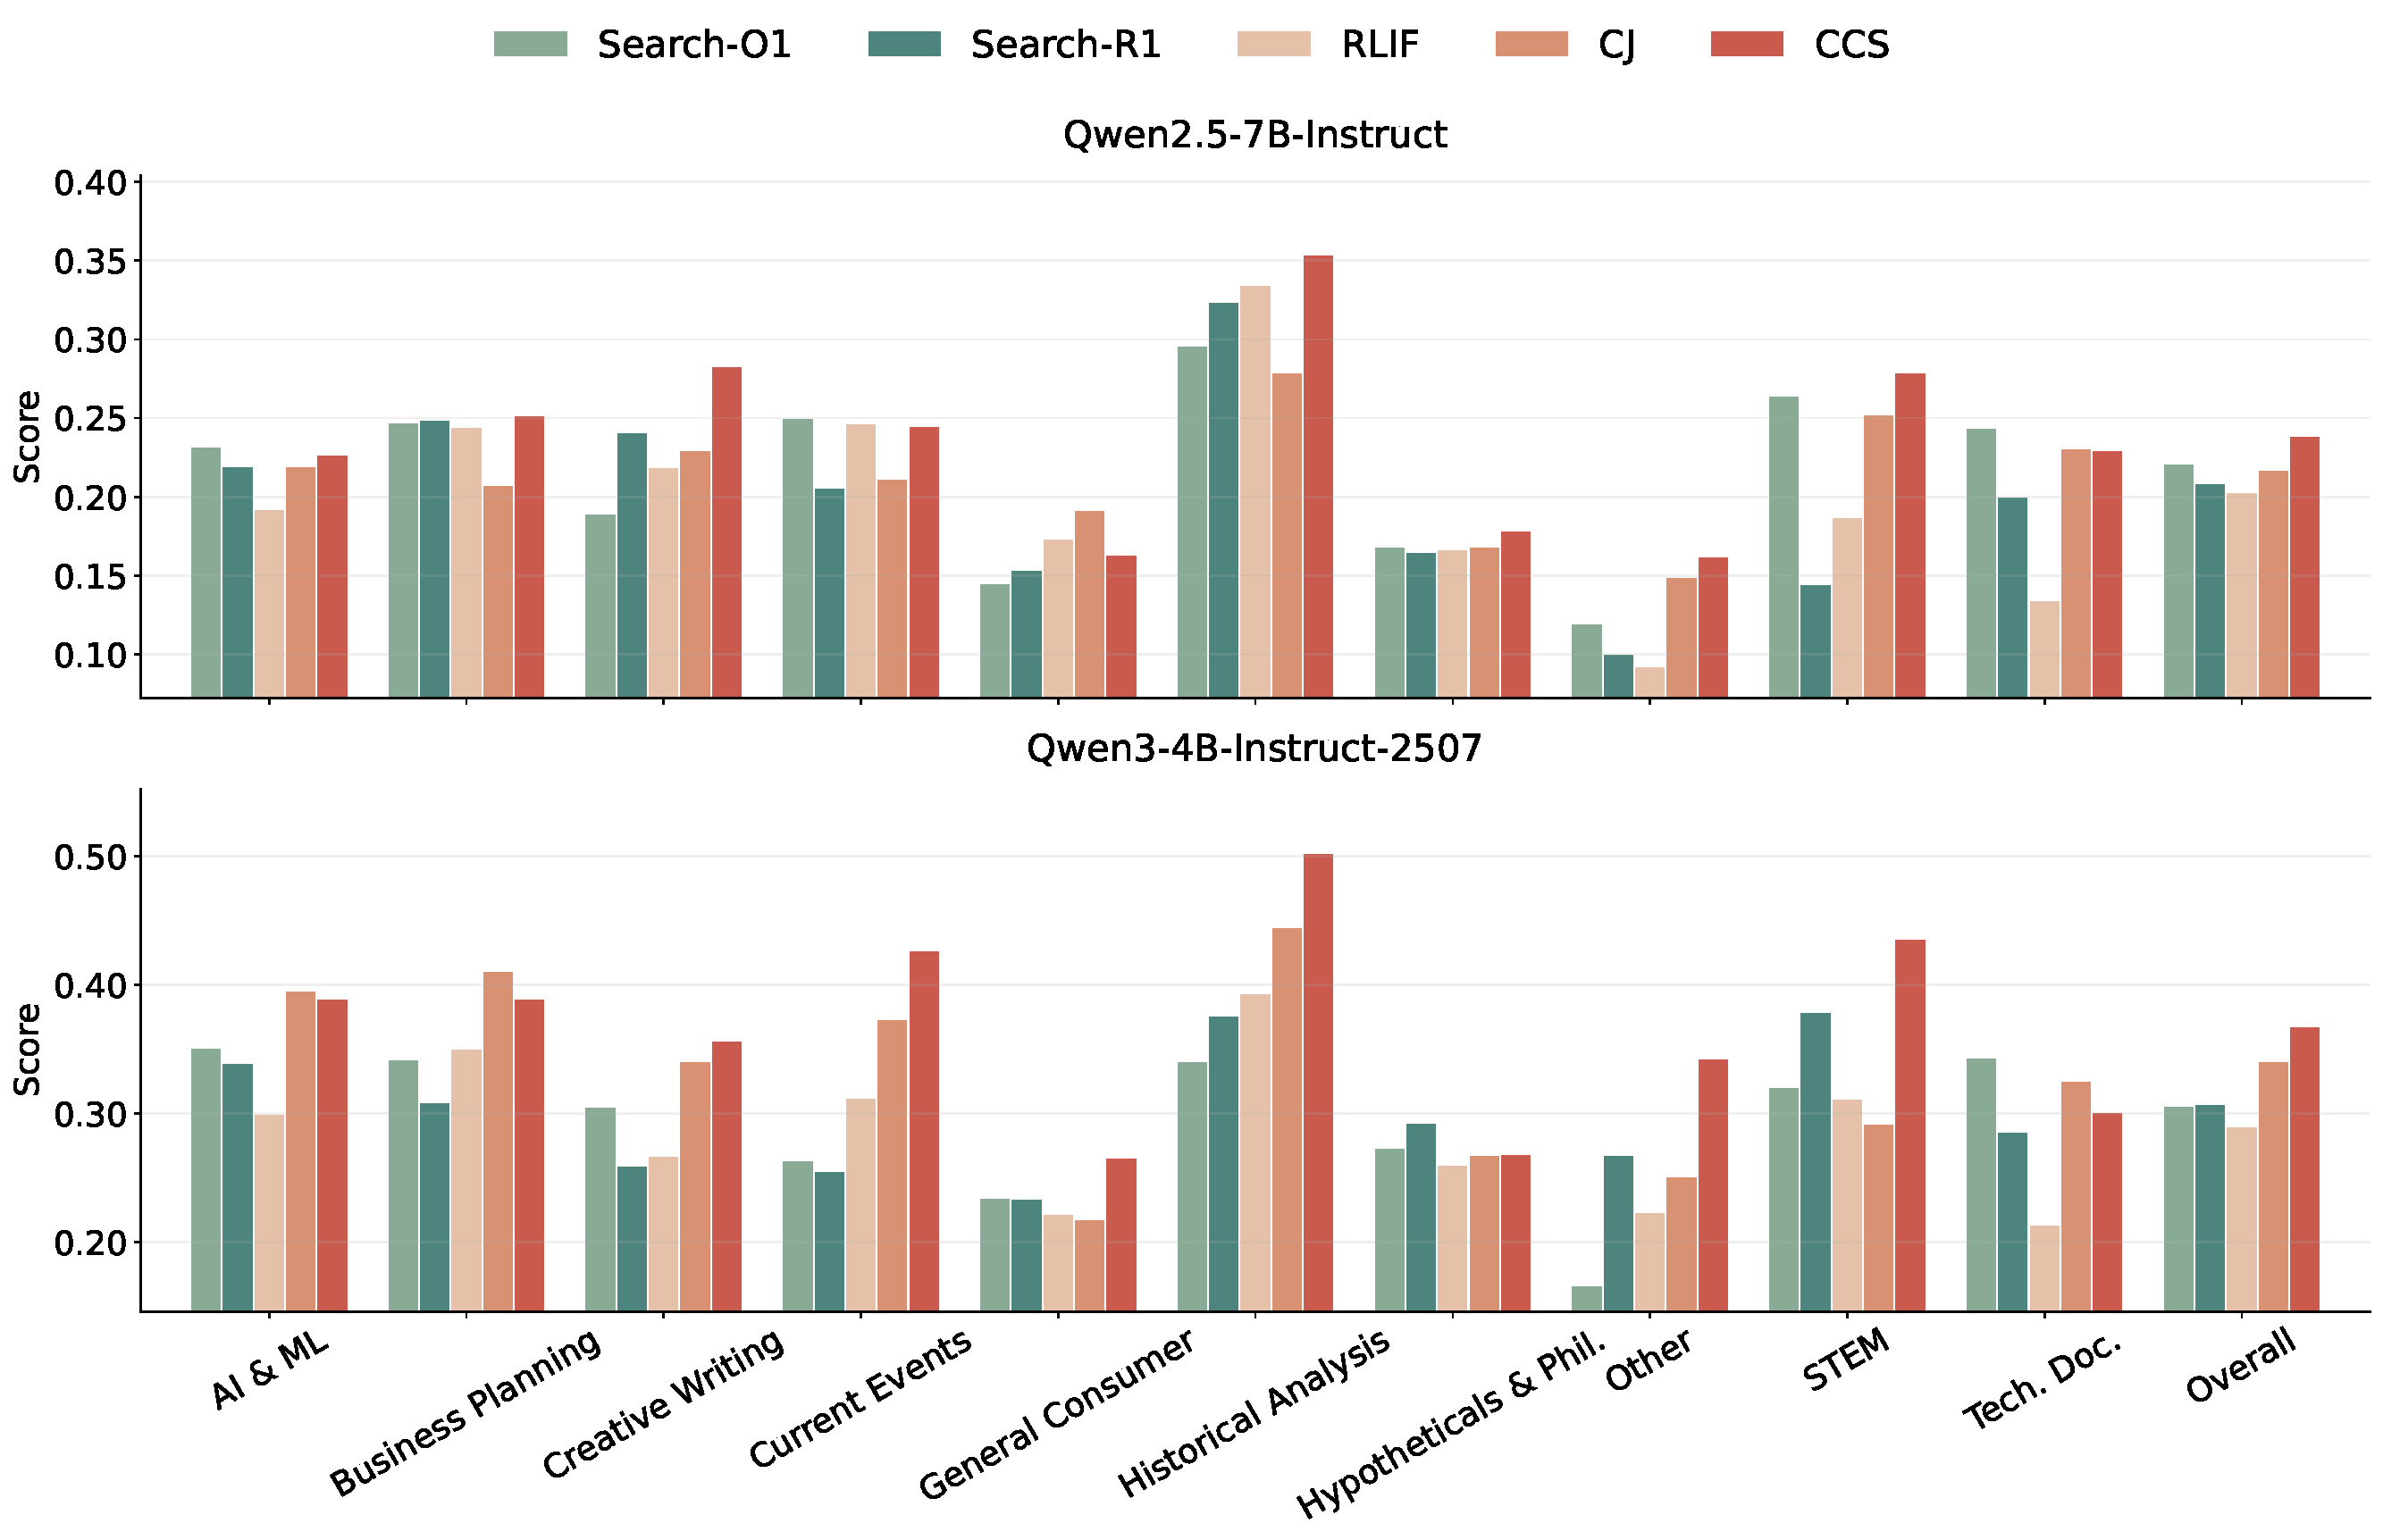
\includegraphics[width=1\linewidth]{img/researchrubrics_results.pdf}
    \caption{\textbf{Performance comparison on the ResearchRubrics \citep{researchrubrics} benchmark for open-ended Deep Research tasks.} Scores are evaluated using the fine-grained rubric-based framework of \citet{researchrubrics}, with Gemini 2.5 Pro as the judge, and are reported as domain-wise scores and the overall average across ten domains.}
    \label{fig:researchrubrics}
\end{figure*}
\subsection{Open-ended Deep Research Task}
Beyond traditional closed-ended question answering tasks, as reported in \Cref{sec:experiments}, we further evaluate CCS on the open-ended Deep Research setting using the ResearchRubrics benchmark \citep{researchrubrics}. This benchmark requires models to integrate multiple capabilities, including the generation of evidence-backed, long-form responses to open-ended queries, and we conduct experiments with Qwen2.5-7B-Instruct and Qwen3-4B-Instruct-2507. Response quality is assessed using the carefully designed fine-grained rubrics introduced by \citet{researchrubrics}, which measure aspects such as factual grounding and clarity, with Gemini 2.5 Pro \citep{comanici2025gemini} serving as the evaluator of model-generated outputs. Notably, ResearchRubrics covers ten diverse domains, including STEM and Historical Analysis. We report both per-domain scores and the overall average score in \Cref{fig:researchrubrics}.

As shown in \Cref{fig:researchrubrics}, CCS achieves the best overall performance on both models, outperforming not only methods that do not rely on gold supervision, but also Search-R1, which is trained with gold supervision. Interestingly, Search-R1, which is optimized to generate ground-truth answers for closed-ended questions, exhibits relatively weaker performance on this open-ended task. More specifically, on Qwen2.5-7B-Instruct, CCS achieves relative improvements of 7.92\%, 14.48\%, 17.63\%, and 9.96\% over Search-O1, Search-R1, RLIF, and CJ, respectively. On Qwen3-4B-Instruct-2507, the corresponding relative improvements are 20.08\%, 19.53\%, 26.81\%, and 7.86\%.